% \documentclass[10pt, english, pdftex]{template/UC3M_document}
\documentclass[10pt, spanish, pdftex]{template/UC3M_document}

\usepackage{listings}

%%%%% Preamble %%%%%
\author{Alejandro Prieto Macías}         % This is me! You should write here your name (for PDF metadata)
%%%%% About the authors (will be used on title page and header) %%%%%

%%% Indicate the number of authors by uncommenting the right option.
\authorstwotrue     % 1 or 2 authors
% \authorsthreetrue   % 3 authors
% \authorsfourtrue    % 4 authors

%%% Fill with the authors data. You can leave empty keys {} if you need to and also if you provide more info that number of authors indicated it will be ignored.
% If you selected \authorstwotrue or \authorsthreetrue (1 to 3 authors)
\authorsuptothree{Alejandro Prieto Macías}{NIA 100383428}{Gr. 81}{Laura Sánchez Cerro}{NIA 100383419}{Gr. 81}{Name3 Lastname3}{NIA 100XXXXXX}{Gr. XX}
% If you selected \coauthorsfourtrue (4 authors)
\authorsfour{Name1 Lastname1}{NIA 100XXXXXX}{Name2 Lastname2}{NIA 100XXXXXX}{Name3 Lastname3}{NIA 100XXXXXX}{Name4 Lastname4}{NIA 100XXXXXX}{Group XX}

%%% If you want to show coauthors email address on the title page, uncomment \emailtrue. Comment it otherwise.
% \emailtrue
% You can leave empty keys {} if you need to and also if you provide more info that number of authors indicated or \emailtrue is commented it will be ignored.
\emails{email1@domain.tld}{email2@domain.tld}{email3@domain.tld}{email4@domain.tld}


%%%%% Basic data about the document (Degree, subject, title, campus, page number custom text) %%%%%
\documentdata{Ingeniería Informática}{Sistemas Distribuidos}{Ejercicio Evaluable 1: Colas de mensajes}{Leganés}{ }

%%%%% Page style %%%%%
\header
\footer
\pagestyle{fancy}

\begin{document}
%%%%% Page title %%%%%
\titleMain

%%%%% Index %%%%%
\begin{spacing}{0.5}
    % \shipout\null                   % Blank page before index (after title page)
    \hypersetup{linkcolor=black}    % References/links on the index will remain black color
    \tableofcontents\newpage        % Index of the document
    % \listoffigures\newpage          % Index of pictures
    % \listoftables\newpage           % Index of tables
\end{spacing}


%%%%% DOCUMENT CONTENT %%%%%
%% VERY IMPORTANT!!! On the first line of this .tex file, select Spanish or English language to coincide with document text language
\section{Introducción}\label{section_label}
El motivo de este ejercicio se basa en la idea de poder aprender las técnicas para poder crear una aplicación cliente-servidor de forma concurrente. Además, se pretende aprender a administrar sistema de comunicación para sistemas distribuidos, es decir, para ordenadores que no comparten el espacio de memoria.

  \vspace{2cm}
  \begin{figure}[h]
    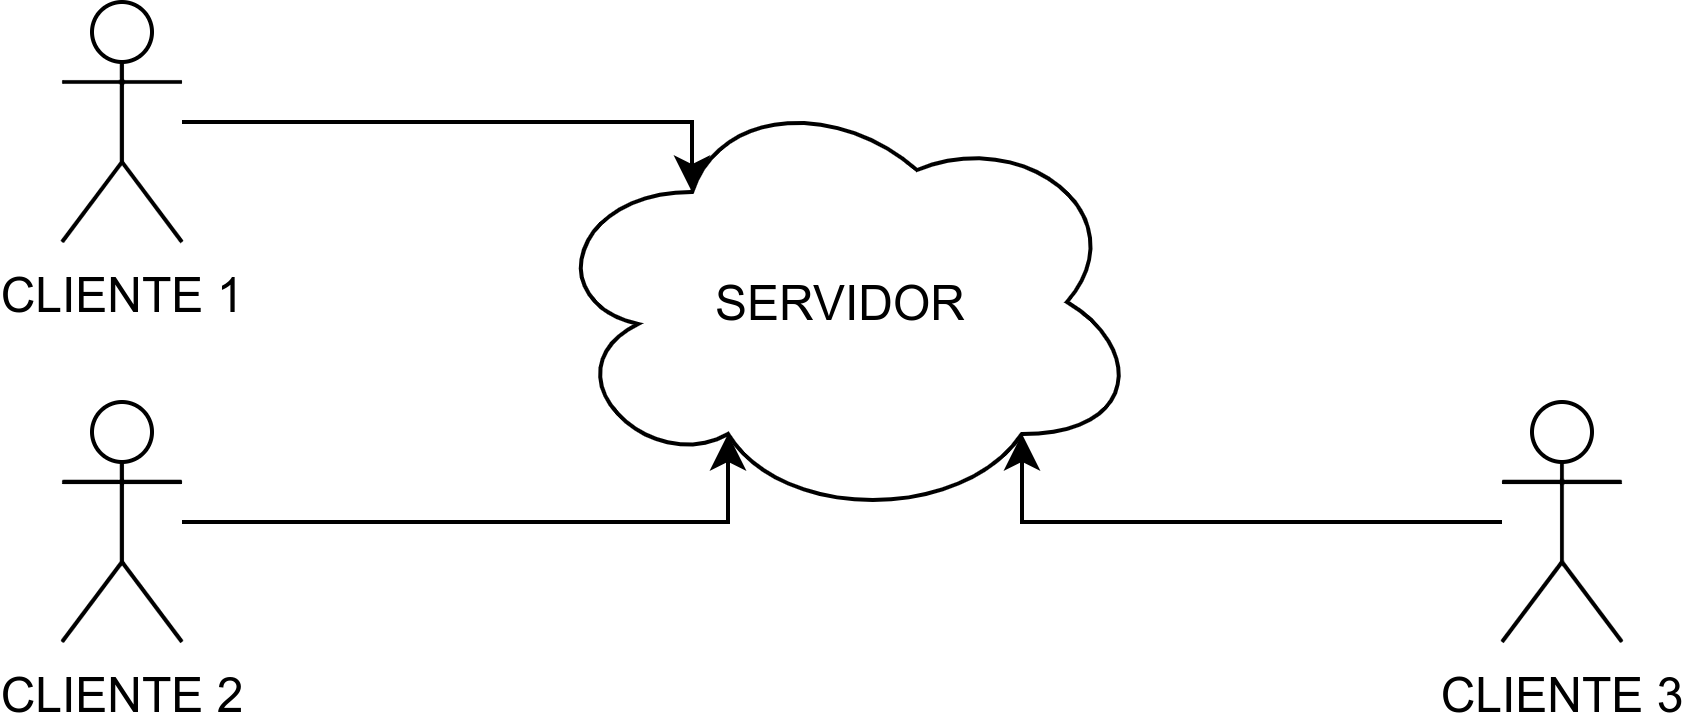
\includegraphics[width=\textwidth]{cliente-servidor.png}
    \caption{Esquema de servicio cliente-servidor concurrente}
    \centering
  \end{figure}


\newpage
\section{Modelo}
Este software pretende que el cliente sea capaz de crear vectores de tamaño N, con un nombre, y poder administrarlos a partir de una aplicación. Estos vectores serán almacenados en el servidor con el que se comunica el cliente.

\subsection{Cliente}
La función del cliente en el sistema es la de utilizar la interfaz gráfica, en este caso el main del archivo \textit{cliente.c} para administrar los datos que el cliente quiere utilizar, es decir, los vectores mencionados anteriormente. Tendrá la capacidades de realizar varias opciones.

\begin{itemize}
  \item \textbf{Crear una vector}: Usará la función \textit{init} para crear el vector especificando el tamaño y longitud a través de los argumentos.
  \item \textbf{Añadir a un vector}: Podrá añadir elementos de tipo número entero al vector a través de esta función indicando la posición en el vector, el nombre del vector y el valor y la función \textit{set}.
  \item \textbf{Obtener de un vector}: Podrá obtener elementos de tipo número entero del vector a través de esta función indicando la posición en el vector, el nombre del vector y el valor y la función \textit{get}.
  \item \textbf{Eliminar un vector}: El cliente, podrá eliminar con la función \textit{destroy} el vector que desee indicando su nombre.
\end{itemize}

\subsubsection{Biblioteca Dinámica}
En la biblioteca dinámica se han implementado las funciones que se comunicarán con el sistema servidor. La inclusión de estructuras de este estilo, es la de facilitar la posible mejora de los sistemas de comunicación sin afectar a la interfaz del usuario, incluso pudiendo tener varias interfaces.

\subsection{Servidor}
El servidor será el encargado de recibir las peticiones y que con ayuda de hilos bajo demanda, se puedan ir ejecutando las acciones que requiere el cliente para administrar los vectores.
El servidor debe estar configurado de tal manera que se evite que se pierdan peticiones debido a condiciones de carrera y por ello, se emplearán herramientas de POSIX para evitarlo. Hemos optado por implementarlo mediante un cerrojo y una variable condicional que hacen que no se pueda atender a una nueva petición si no se atendió a la anterior. El término atender, no se refiere a procesar la petición, simplemente al hecho de copiar la petición de entrada en una variable local y evitar que se pierda.

\subsection{Servidor Pool de Hilos}
Se ha implementado también la versión con un pool de hilos que consiste en crear un número de hilos determinados. Cada vez que llega una nueva petición se almacena en una cola circular de tareas y serán los hilos los que se encargan de recoger y procesar esas tareas cuando puedan actuar. Se trata de una versión del problema de \textit{productor-consumidor} en el que produce el hilo principal y los hilos que se crean son los que consumen de la cola circular.

Para su compilación:
  \begin{lstlisting}[frame=single]
    make servidorPool
  \end{lstlisting}


\subsubsection{Modelo de datos}
Para administrar la pequeña base de datos que almacena los vectores, se ha decidido establecer una lista enlazada implementada a través de un \textit{struct} del lenguaje de programación \textbf{C}. Cada elemento de la lista está formado por un vector de tamaño N, una cadena de caracteres y el puntero al siguiente elemento.
Además, las peticiones se han podido realizar mediante \textit{structs} debido a la tecnología de comunicación que son las colas de mensajes del sistema UNIX.

\subsubsection{Implementación}
Las funciones que manejan la lista enlazada se encuentran en un archivo distinto al del propio servidor para facilitar los cambios en el sistema, dando prioridad a la modularización del sistema. Las funciones que realizan los clientes tienen su correspondencia en el servidor.
\begin{itemize}
    \item \textbf{Crear una vector}: La función \textit{INIT} será la encarga de crear un nuevo elemento en la lista, para ello se debe reservar en memoria el tamaño necesario para almacenar un vector de N enteros, la cadena de caracteres de tamaño \textbf{MAX} (que se establece en 100 caracteres) y el puntero. Además, se deberá enlazar con el elemento correspondiente.
    \item \textbf{Añadir a un vector}: La función \textit{SET} se encargará de encontrar el vector a través del nombre en la lista y posteriormente se encargará de cambiar el valor que se almacenaba en la posición indicada por el valor que se desea introducir.
    \item \textbf{Obtener de un vector}: La función \textit{GET} de encontrar el vector a través del nombre en la lista y posteriormente se encargará de mostrar el valor que se almacenaba en la posición indicada.
    \item \textbf{Eliminar un vector}: La función \textit{DESTROY} se encarga de eliminar el espacio de memoria que ocupaba el vector en la lista y, además, enlazar correctamente los elementos de lista para evitar que queden elementos sin apuntar.
\end{itemize}


\newpage
\section{Conclusiones}
Esta práctica nos ha permitido aprender la estructura básica de un sistema de tipo cliente-servidor, pudiendo descubrir algunas de sus ventajas y desventajas.

\begin{itemize}
  \item \textbf{Ventajas}
    \begin{itemize}
      \item Modularidad.
      \item Menor cómputo en los dispositivos de los clientes.
    \end{itemize}
  \item \textbf{Desventajas}
  \begin{itemize}
    \item Mucha dependencia de los servidores.
    \item Puede llegar a colapsar el sevicio si llegan demasiadas peticiones.
  \end{itemize}
\end{itemize}

Por otro lado, hemos tenido ciertas dificultades a la hora de realizar la concurrencia puesto que la implementación con un \textit{pool de hilos} que permite hacer mucho más eficaz el sistema evitando que se lancen muchos más hilos llegando incluso a poder empeorar la calidad del servicio. Decidimos empezar la tarea con \textit{hilos bajo demanda} y resultó menos complejo, tras completar esta versión pudimos realizar la versión con el \textit{pool de hilos}.


\end{document}
